\section{Styrhandske}
\begin{figure}[H]
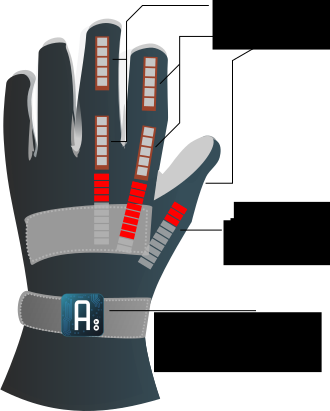
\includegraphics[height=0.5\textheight]{img/kontrollhandske}
\caption{Konceptskiss över styrhandsken. Röda ledlampor indikerar hur högt }
\end{figure}
%Detta är intro. Det ska inte vara några detaljer här, bara översiktligt!
% Konvention: styrhandske, inte reglerhandske eller kontrollhanske

För att intuitivt reglera robothanden används en tunn handske som användaren bär på sin hand. På handskens tumme, långfinger och pekfinger finns det två flexsensorer vardera som följer användarens hand och ändrar resistans beroende på hur mycket de böjs. Resistansen samplas av en mikrokontroller, som efter filtrering trådlöst sänder styrsignaler till robothanden.
Robothanden sänder i sin tur trycket från dess fingrar till styrhandsken. Trycket återkopplas till användaren genom att fler ledlampor på handen tänds ju större trycket är.


\comment{Emil: Skriv om handens fysiska konstruktion}

\comment{öjeling: fin bild hur signaler åker runt}

\comment{Kanske något enkelet schema för hur det är uppkopplat}




\section{Algoritmer}
Här presenteras de styralgortimter som bestämmer hur handen beter sig när den följer användarens input samt identifierar och greppar objekt. 


\section{Objektidentifiering}
\begin{figure}[H]
EN BILD SOM FÖRKLARAR DETTA, SAMT VILKA OBJEKT VI VALT ATT identifierar och hur vi gör det...
\caption{Beskrivning}
\end{figure}
Antaganden: Servona står i önskat läge, det vill säga tidsfördröjningen som uppstår då servona skall vrida sig från godtycklig position till den önskade antags vara så liten vid normalt användande att den kan försummas. Då ingen mätning av servonas verkliga position görs, är den enda informationen om fingrarnas lägen det önskade servoläget. 

FIXA FLÖDESSSCHEMA OCH ETT ARDUINO PROGRAM Känner av tryck (över visst gränsvärde) på tumme och motstående finger->, lagrar användarens input läge då detta inträffar ( för att när användaren går utanför detta igen (öppnar sin hand) så skall handen återgår till att följa användaren) -> beräknar avståndet mellan sensorerna-> checkar av avståndet mot en lista av fördefinerade objekt som innehåller , storlek och önskat trycksensorvärde med en +/-tolerans för att inte handen ska stå och flippa som en tok för att uppnå EXAKT rätt värde-> TADAA!!-> när användaren öppnar sina fingrar utanför ``kontaktläget'' följer handen efter igen...
Mer teksti
